\documentclass{beamer}
\usetheme{Singapore}

\usepackage[utf8]{inputenc}
\usepackage{tikz}
%\usetikzlibrary{patterns}
\usetikzlibrary{shapes.geometric}
\usetikzlibrary{calc}
%\usetikzlibrary{automata,positioning}
\usepackage{siunitx}
\usepackage[e]{esvect}

\usepackage{array}
\usepackage{chemfig}
\usepackage{amsmath}
\usepackage{amssymb}
%\usepackage[cal=boondoxo]{mathalfa} 
%\usepackage{enumitem}
%\usepackage{lastpage}
\usepackage{tcolorbox}
%\usepackage{siunitx}

\title{Chapitre 6 : Le mouvement}
\author{ROSALIE}
\date{2024}

\renewcommand{\arraystretch}{1.5}
\setbeamersize{text margin left=3mm,text margin right=3mm}


\begin{document}
\title{\textbf{Présentation aux parents}}
\author{ROSALIE Rémy}
%\date{\today}
% Title page frame
\begin{frame}
\titlepage
\end{frame}

\begin{frame}
	\frametitle{Le Baccalauréat}
    \begin{center}
        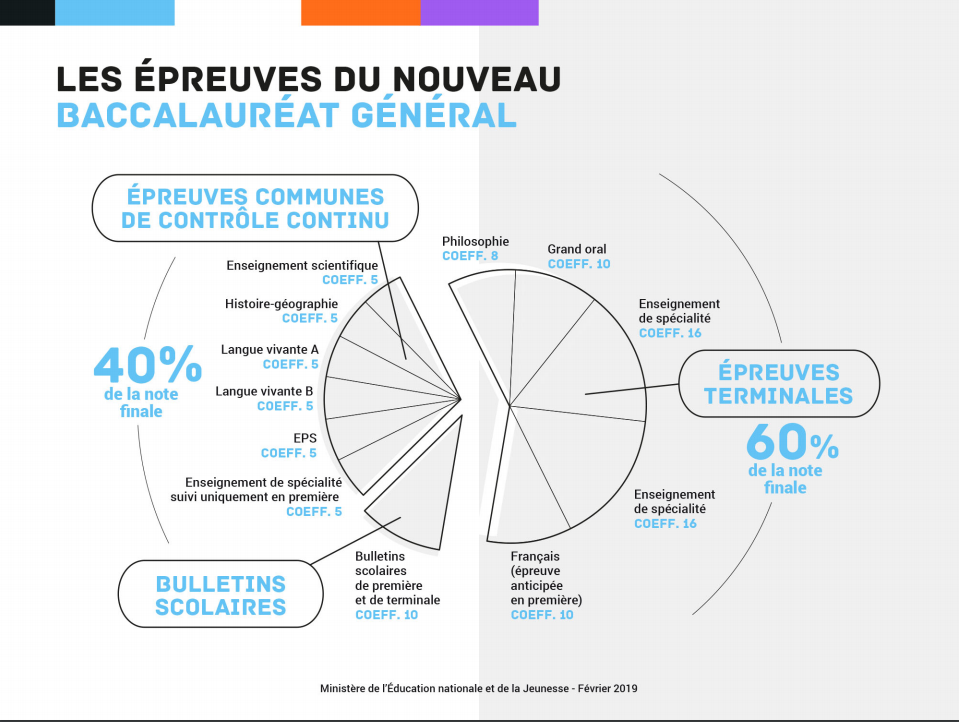
\includegraphics[width=.9\paperwidth]{CoefBac.png}
    \end{center}
\end{frame}

\begin{frame}
	\frametitle{La vie en première}
    \centering
        \begin{minipage}{.25\paperwidth}
        
\includegraphics[width=\linewidth]{Organisation.png}
        \textbf{Organisation}
        \end{minipage}\hspace{.25\paperwidth}
        \begin{minipage}{.25\paperwidth}
            
\includegraphics[width=\linewidth]{Travail personnel.png}
            \textbf{Travail Personnel}
        \end{minipage}

        \begin{minipage}{.25\paperwidth}
            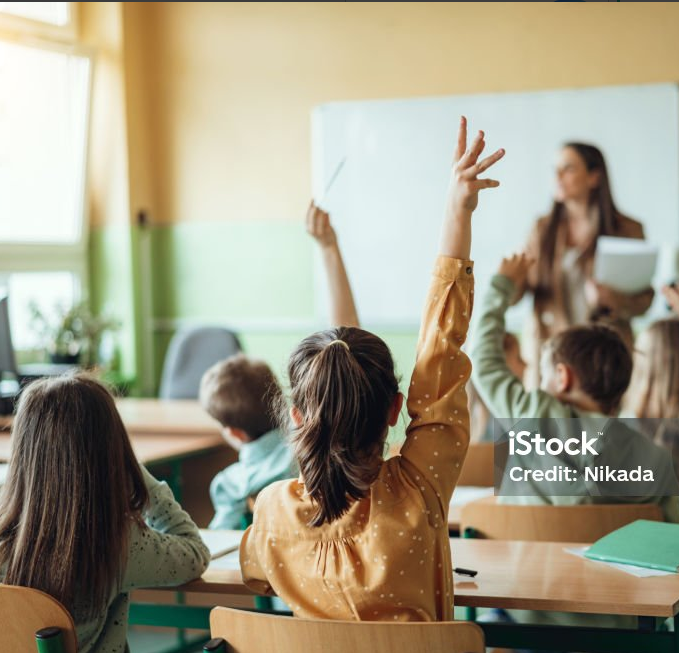
\includegraphics[width=\linewidth]{Participation.png}
            \textbf{Participation}
            \end{minipage}\hspace{.25\paperwidth}
        \begin{minipage}{.25\paperwidth}
            
\includegraphics[width=\linewidth]{Esprit critique.png}
            \textbf{Esprit critique}
        \end{minipage}
\end{frame}

\begin{frame}
	\frametitle{Orientation}
    \begin{center}
        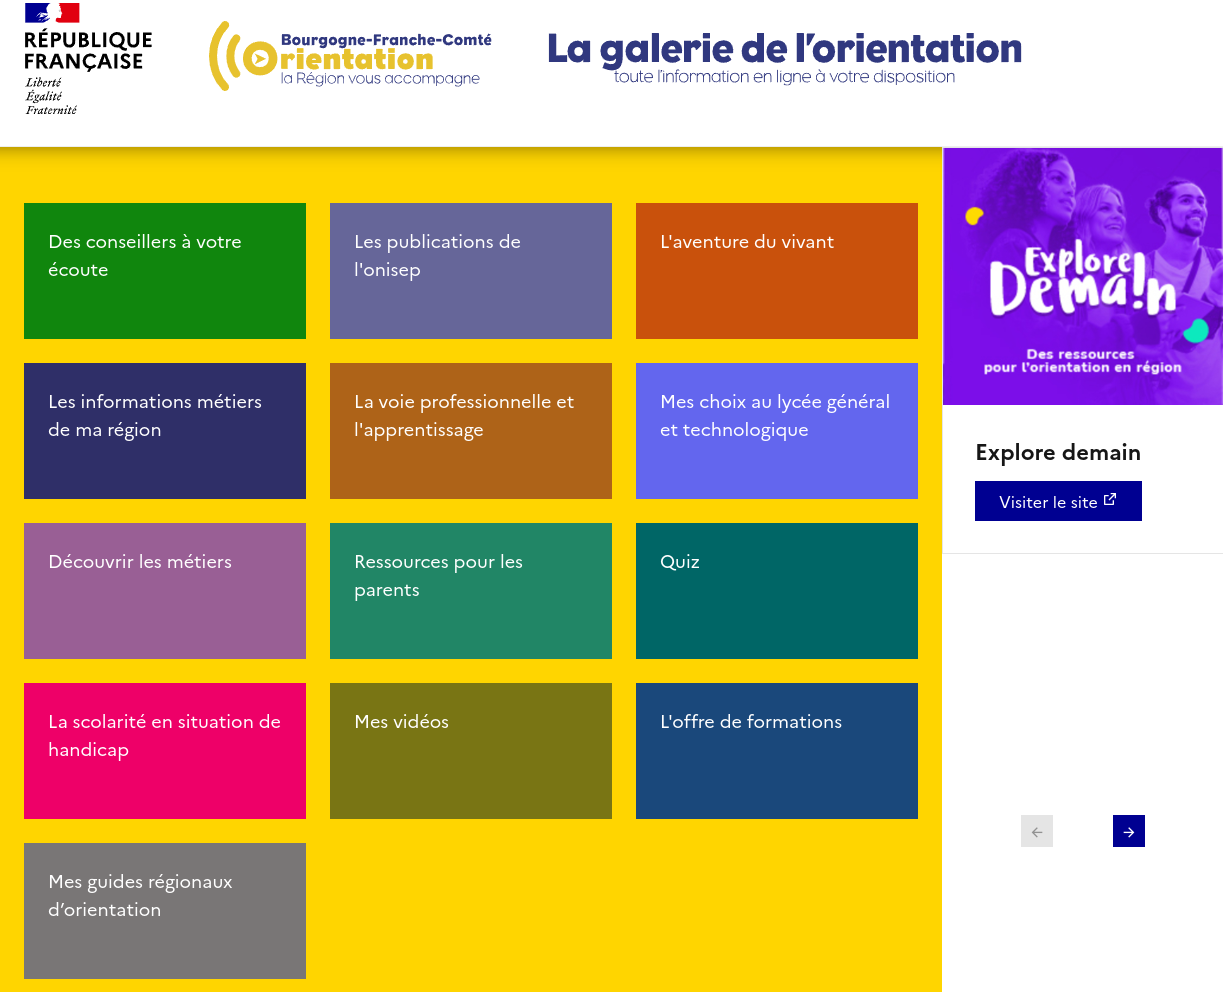
\includegraphics[width=.9\paperwidth]{Orientation.png}
    \end{center}
\end{frame}


\end{document}